\section{Frontend}
\rhead{Frontend}

A frontend a szoftver azon része, amely nagyban meghatározza egy felhasználó élményét. Fontos az átláthatóság, a könnyű kezelhetőség és az esztétika. Ezen szempontokat figyelembe véve készítettük el az Archytex weboldalt.

\subsection{Dizájn terv}
A honlap elkészítésének első lépése a tervezés volt. Ehhez a Figma\footnote{\url{https://www.figma.com/}} nevű ingyenes dizájn szoftvert használtuk. Ezen alkalmazás segítségével könnyedén tudtunk vázlatot készíteni arról, hogy hogyan képzeljük el a honlap megjelenését, még azelőtt, hogy elkezdtük volna a programozást.

A Figma a dizájn tervezés mellett használható vektor grafikák rajzolására is, amellyel az Archytex szerkesztőben látható ikonok készültek.

\begin{figure}[H]
  \centering
  
\includegraphics[width=0.1\textwidth]{parts/developer-documentation/frontend/images/meshSelectMode.png}
  
\includegraphics[width=0.1\textwidth]{parts/developer-documentation/frontend/images/faceSelectMode.png}
  
\includegraphics[width=0.1\textwidth]{parts/developer-documentation/frontend/images/vertexSelectMode.png}
  \caption{Példa a Figma-ban készíthető vektor grafikákra: a kiválasztási módok ikonjai az Archytex szerkesztőből.}
\end{figure}

A honlapon megjelenő grafikák egy része az Undraw\footnote{\url{https://undraw.co/}} nevű honlapon található, ingyenesen használható illusztrációk felhasználásával készült. Ezen illusztrációk nyílt licenccel rendelkeznek, ezért szerkeszthetőek és ingyenesen felhasználhatóak. Néhány grafikát a Figma-ban szerkesztettünk, hogy több építészeti elemet tartalmazzanak, vagy hogy jobban illeszkedjenek a dizájn környezetbe.

Az Archytex logó is a Figma beépített vektor grafikai eszközeivel készült. A dizájn követi a letisztultság elvét, és használja a honlap elsődleges színét. A logó sötét és világos módtól függően a honlapon megváltozik a jobb láthatóság érdekében.

\begin{figure}[H]
  \centering
  
\includegraphics[width=0.1\textwidth]{parts/developer-documentation/frontend/images/logo.png}
  \caption{Az Archytex logó}
\end{figure}

\subsection{Használt technológiák}
A frontend alkalmazás React-ben\footnote{\url{https://hu.reactjs.org/}} készült. Azért esett a választás erre a keretrendszerre, mert a horog alapú komponens állapot- és életcikluskezelése miatt fejlesztői élményét tekintve kiemelkedően jobb, mint más rendszerek. Emellett az is segítette a választást, hogy jelenleg a React a legnépszerűbb a webfejlesztők köreiben\cite{most-used-web-frameworks}, ezért rengeteg forrás és oktatóvideó érhető el hozzá.

A honlap elkészítéséhez a Material UI (MUI)\footnote{\url{https://mui.com/}} nevű komponens könyvtárat használtuk, amely rengeteg előre elkészített és könnyen testreszabható komponenst tartalmaz. Ennek segítségével és a Google által kifejlesztett Material Design\footnote{\url{https://material.io/}} irányelveit követve modern, letisztult és felhasználóbarát felületet tudtunk létrehozni.

A csomagkezeléshez \emph{yarn}-t használunk, amely az \emph{npm} csomagkezelő népszerű alternatívája.

\subsection{Reszponzivitás}
Egy modern holnap készítésénél elengedhetetlen, hogy minden eszközön használható legyen, bármilyen megjelenítőt támogasson. Az Archytex honlapon a reszponzivitás megvalósításában a MUI könyvtár segít. A Container és a Grid komponensek egyszerűen testreszabhatók a különböző töréspontokon. Emellett azon komponensek esetében, ahol szükség van a töréspontokkal kapcsolatos logikára, ott a useMediaQuery horog nyújt megoldást.

\begin{figure}[H]
  \centering
  
\includegraphics[height=7cm]{parts/developer-documentation/frontend/images/mobile-view.png}
  \caption{Navigációs menü mobil nézetben}
\end{figure}

\subsection{Főoldal}
A főoldal célja, hogy egy új felhasználónak "eladja" a termékünket. Ezért fontos volt, hogy látványos és emlékezetes legyen, de ezek mellett egyben informatív is. A látványossághoz nagyban hozzájárultak az Undraw.io-s illusztrációk és a tsparticles\footnote{\url{https://github.com/matteobruni/tsparticles/tree/main/components/react}} JavaScript könyvtár segítségével létrehozott, az oldal fejlécében megjelenő interaktív buborékok. Emellett az interaktivitás növelése érdekében az AOS (Animate On Scroll) könyvtárat használva megoldottuk, hogy a honlap tartalma folyamatosan jelenjen meg, ahogy a felhasználó görget lefelé a honlapon.

\begin{figure}[H]
  \centering
  
\includegraphics[width=\textwidth]{parts/developer-documentation/frontend/images/header.png}
  \caption{Az Archytex főoldal fejléce}
\end{figure}

\subsection{Autentikáció}
A bejelentkezési és regisztrációs képernyő frontend funkcionalitás szempontjából egy viszonylag nagyobb kihívást nyújtott, mint más oldalak. Tudtuk, hogy gyakran lesz szükségünk olyan űrlapokra a projekt folyamán, amiben a felhasználó felé visszajelzést kell küldeni, ezért készítettünk egy generalizált React komponenst ennek a feladatnak az ellátására. Ezzel beviteli mező komponenssel már könnyedén fel tudtunk építeni mind a bejelentkezési és a regisztrációs űrlapot, és a hibakezelés sem okozott problémát.

\begin{figure}[H]
  \centering
  \begin{minipage}{.5\textwidth}
    \centering
    
\includegraphics[width=.6\linewidth]{parts/developer-documentation/frontend/images/login.png}
    \label{fig:loginPage}
  \end{minipage}%
  \begin{minipage}{.5\textwidth}
    \centering
    \begin{lstlisting}
      <FormInput
        variant='username'
        label={t("username")}
        input={username}
        inputChange={handleUsernameChange}
        error={usernameError}
      />\end{lstlisting}
  \end{minipage}
  \caption{Példa az egyedi beviteli komponens használatára a bejelentkezési képernyőn}
\end{figure}

\pagebreak

\subsection{Irányítópult}
Az Archytex irányítópult feladata a projektek listázása és egy felhasználói interfész biztosítása ezen projektek beállításainak módosítására, tulajdonságaik megtekintésére. Egy projekten belül megjelennek a projekthez tartozó renderek, amik letölthetőek és kinagyíthatók.

A projektek lekérése és tárolása saját szolgáltatás segítségével történik. Ez a szolgáltatás tartalmazza a projektet és a rendert jellemző modellként szolgáló TypeScript interfészeket. Emellett a useState és a useContext horgokat használva eltárolja az API-val lekért adatokat, amik utána egy egyedi horog (useProjects) segítségével érhetők el a célkomponensben.

\subsection{Szerkesztő UI}
A szerkesztő és a frontend közötti kommunikáció egy egyedi API segítségével történik. Beállítható ezen keresztül a szerkesztőben a transzformációs mód\footnote{Transzformációs mód: lap, él, csúcs vagy díszítőelem kiválasztása}, és kiválasztható a használni kívánt textúra és a díszítőelem. A jelenlegi mód állapotát a szerkesztő gyökérkomponense kezeli, és innen adja át a MUI-s \emph{ToggleButtonGroup}-ra épített gomb csoport komponensnek. Ezáltal a gombok megnyomásával is állítható a transzformációs mód.

\subsubsection{Könyvtár ablak}
A textúra és a díszítőelem kiválasztására a könyvtár ablak komponens szolgál. Ez egy modál ablak, amely MUI komponenseket és egy saját szolgáltatást használva megjeleníti az elérhető textúrákat vagy díszítőelemeket. A könyvtárban minden elem rendelkezik egy névvel és egy vagy több tulajdonsággal, amik Chip komponens formájában jelennek meg az elem kártyáján. A név és minden tulajdonság szűrhető, így elősegítve a könnyebb keresést.

\begin{figure}[H]
  \centering
  \begin{minipage}{.5\textwidth}
    \centering
    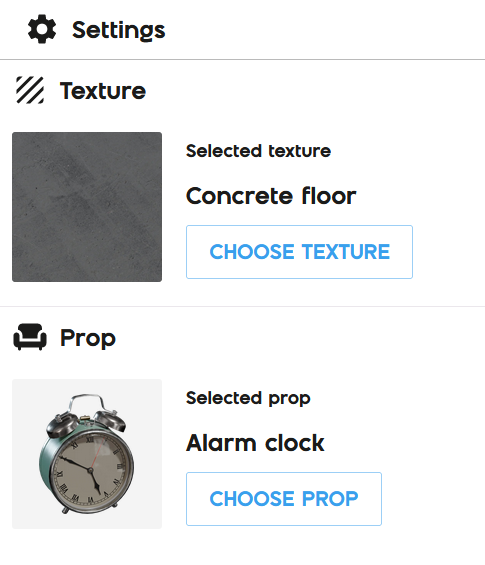
\includegraphics[width=.6\linewidth]{parts/developer-documentation/frontend/images/editorSettings.png}
    \label{fig:editorSettings}
  \end{minipage}%
  \begin{minipage}{.5\textwidth}
    \centering
    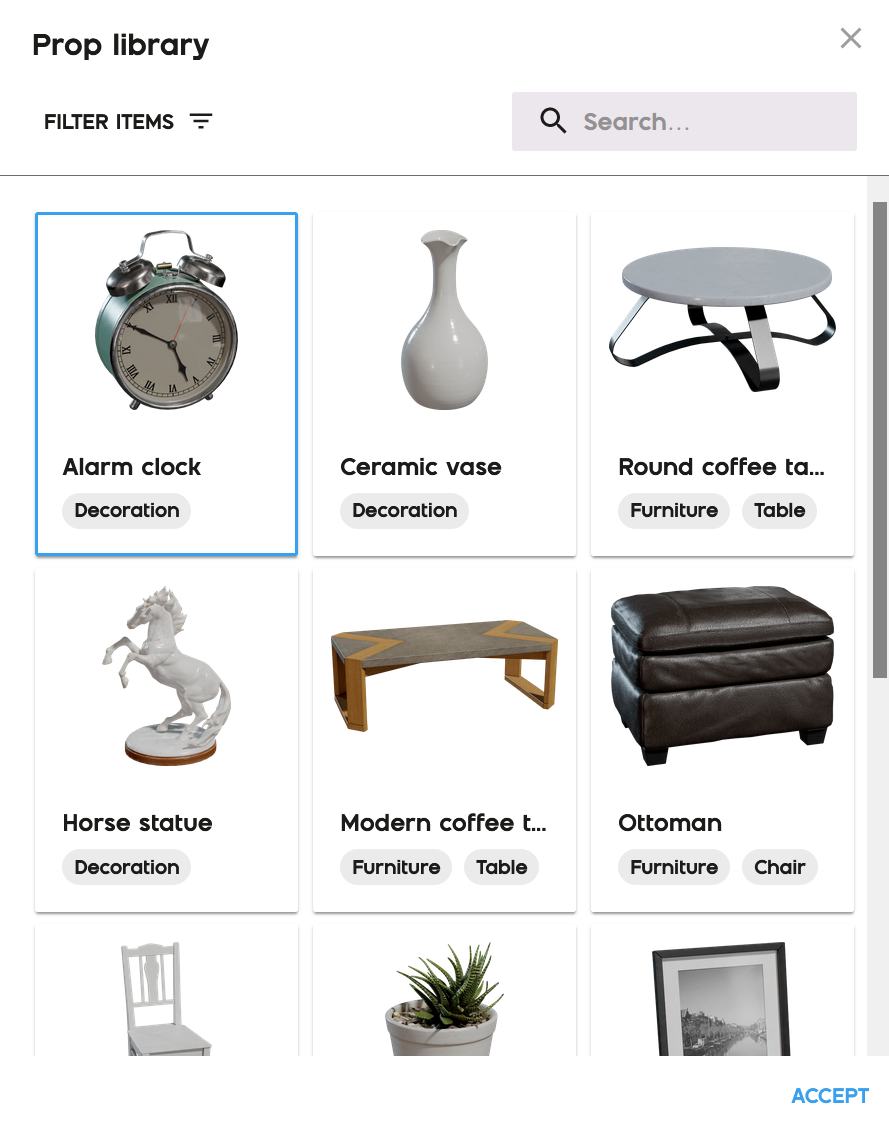
\includegraphics[width=.6\linewidth]{parts/developer-documentation/frontend/images/library.png}
    \label{fig:library}
  \end{minipage}
  \caption{Szerkesztő beállítások és a díszítőelem könyvtár ablak}
\end{figure}

\subsection{Fordítások}
Az Archytex alkalmazás több nyelven is elérhető. Az i18n\footnote{i18n: Internationalisation, avagy nemzetköziesítés}  megvalósításához az i18next nevű React könyvtárat használtuk. Az alkalmazás gyökérkomponensében importáltuk az nyelvekhez tartozó JSON fájlokat, amikben megtalálható az összes előforduló fordítási kulcs, amelyhez tartozik egy-egy hozzárendelt fordítás.

\begin{figure}[H]
  \centering
  \begin{minipage}{.7\textwidth}
    \centering
    \begin{lstlisting}
      i18n.use(initReactI18next).init({
        resources: {
          en: { translation: translationEn },
          hu: { translation: translationHu },
          jp: { translation: translationJp },
        },
        lng: "en",
        fallbackLng: "en",
        interpolation: { escapeValue: false },
      });\end{lstlisting}
  \end{minipage}
  \caption{Az i18next inicializálása angol, magyar és japán nyelvvel}
\end{figure}

\begin{figure}[H]
  \centering
  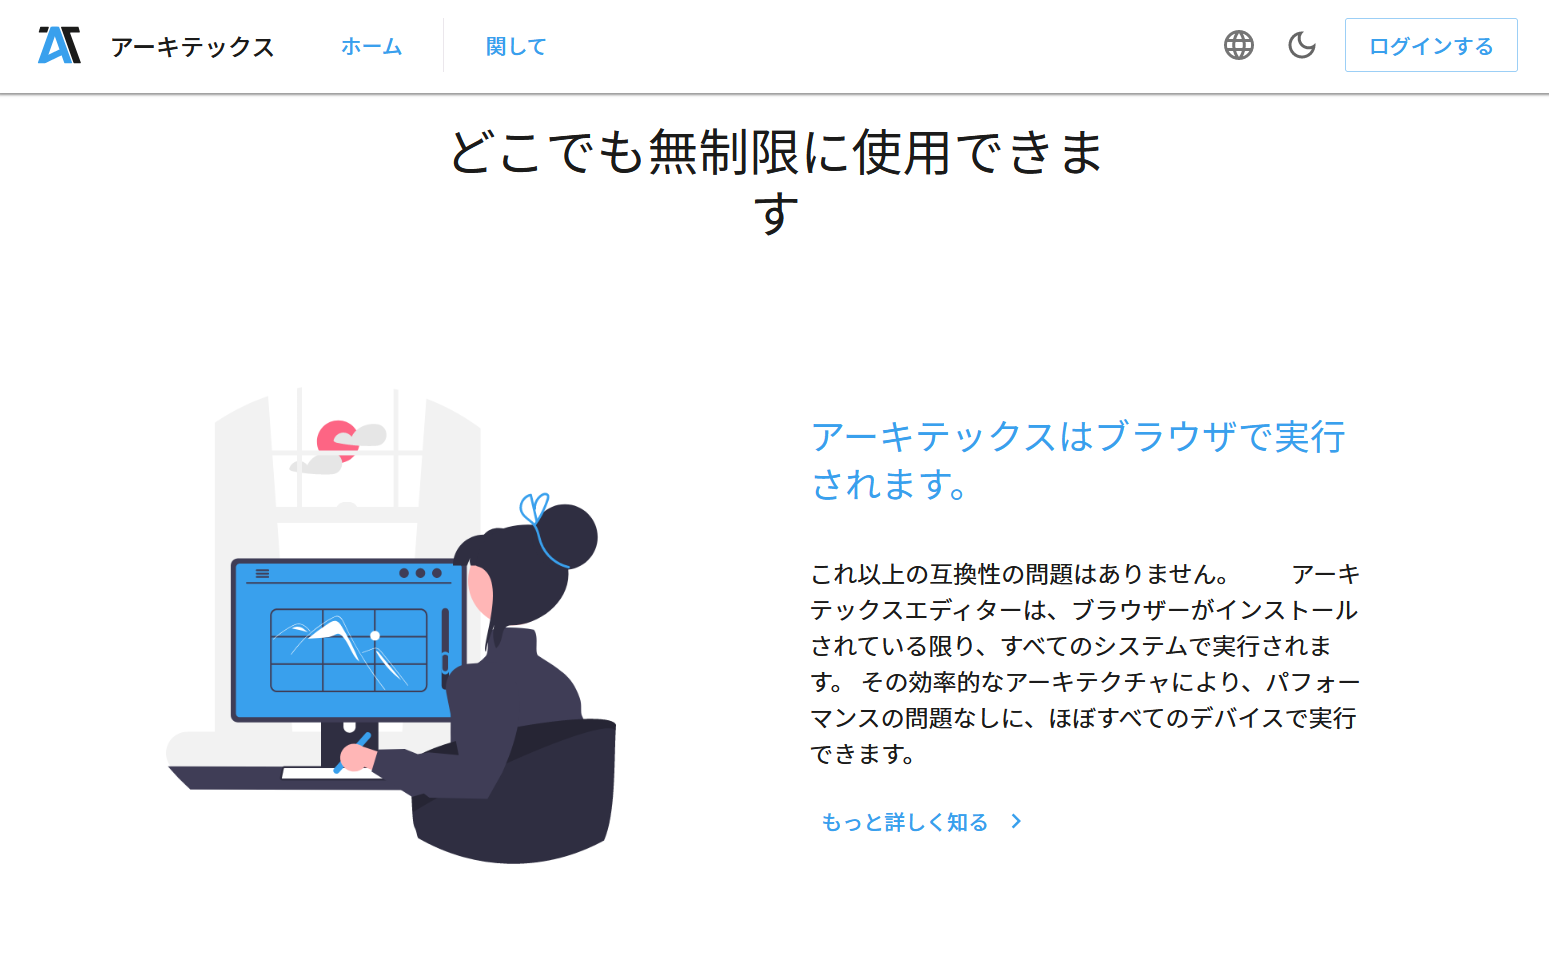
\includegraphics[width=.6\textwidth]{parts/developer-documentation/frontend/images/translated.png}
  \caption{Az Archytex főoldal egy bekezdése japán nyelven}
\end{figure}

\subsection{Tesztek}
\todo{Write subsection}